% !TEX root = main_memo.tex

\chapter{Introduction}


\begin{definition}\label{MainDef}
Given topological spaces $X,X', Y, Y'$,
we say that a function $f:X\rao Y$ \emph{continuously reduces}\index[IdxNotion]{continuous reduction!between functions}
to a function $g:X'\rao Y'$ if there are two continuous functions $\sigma:X\rao X'$
and $\tau:\im(g\circ\sigma)\rao\im(f)$ such that $f=\tau\circ g\circ\sigma$. In this case, we write $f\leq g$ and say that the pair $(\sigma,\tau)$ \emph{continuously reduces}, or simply \emph{reduces}, $f$ to $g$.
\end{definition}

\begin{center}
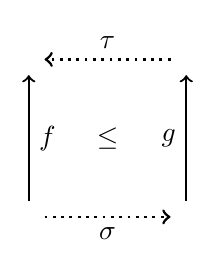
\begin{tikzpicture}[line width=1pt]

\def \Side{2}
\def \p{0.2}
\draw[->, dotted] (\p,0) -- ({\Side-\p},0) node[midway,below] {$\sigma$};

\draw[->, dotted] ({\Side-\p},\Side)-- (\p,\Side)  node[midway,above] {$\tau$};
\draw[->, thick] (0,\p) -- (0,{\Side-\p}) node[midway,right] {$f$};
\draw[->, thick] (\Side,\p) -- (\Side,{\Side-\p})  node[midway,left] {$g$};
\draw (0.5*\Side,0.5*\Side) node    {$\leq$};

\end{tikzpicture}
\end{center}


Continuous reducibility is a transitive and reflexive relation, namely a \emph{quasi-order}\index[IdxNotion]{quasi-order}.
As usual with quasi-orders, there is an induced equivalence relation: we write $f\equiv g$ when both $f\leq g$ and $g\leq f$ hold,
and we say that $f$ and $g$ are \emph{continuously equivalent}\index[IdxNotion]{continuous reducibility!induced equivalence relation}.
We also denote by $f<g$\index[IdxSymb]{0@{$f\leq g$, $f<g$, $f\equiv g$}} the relation $f\leq g$ and $f\not\geq g$, and we say that $f$ and $g$ are \emph{incomparable} \index[IdxNotion]{incomparable}%{Continuous reduction!Incomparability} 
when both $f\not\leq g$ and $g\not\leq f$.

An \emph{antichain}\index[IdxNotion]{antichain} is a set of pairwise incomparable elements, and an \emph{infinite strictly descending chain} is a sequence $(f_n)_{n\in\N}$
satisfying $f_{n+1}<f_n$ for all $n\in\N$. A quasi-order is called a \emph{well-quasi-order}\index[IdxNotion]{well-quasi-order (\wqo{})}, or \wqo{}, if it has no infinite antichains and no infinite descending chains.

A topological space is \emph{Polish}\index[IdxNotion]{space!Polish} if it is separable and completely metrizable, and \emph{zero-dimensional}\index[IdxNotion]{space!zero-dimensional} if it has a basis consisting of \emph{clopen sets},
that is sets that are both open and closed. A topological space is \emph{analytic}\index[IdxNotion]{space!analytic} if it is a continuous image of a Polish space.

Our main result is the following theorem.

\begin{maintheorem}\label{MainTheorem1}
Continuous reducibility is a well-quasi-order on the class of continuous functions from an analytic zero-dimensional space to a separable metrizable space.
\end{maintheorem}

The analyticity hypothesis in \cref{MainTheorem1} is only used to show that all such continuous functions with uncountable image are equivalent to the identity function on the Cantor space. In fact, we prove

\begin{maintheorem}\label{MainTheorem2}
Continuous reducibility is a well-quasi-order on the class of continuous functions from a separable metrizable zero-dimensional space to a countable metrizable space.
\end{maintheorem}

The above theorem is proved following a dichotomy which is reminiscent of the case of spaces.
Recall that a space is \emph{scattered}\index[IdxNotion]{space!scattered}\index[IdxNotion]{scattered!space} if any of its non-empty subsets contains an isolated point. We suggest to make the following definition:
a function $f$ between topological spaces is \emph{scattered}\index[IdxNotion]{scattered!function}\index[IdxNotion]{function!scattered} if any non-empty subset of its domain contains a {non-empty} open set on which $f$ is constant.
Every continuous function with a scattered image is scattered, but scattered continuous functions may have a non scattered image (for example, any bijection $:\N\to\Q$) or domain (for example, a constant function on $\Q$).

While the space $\Q$ of rationals is universal for countable metrizable spaces, any non scattered metrizable space contains a copy of $\Q$.
We show analogous results for functions with $\id_\Q$, the identity on $\Q$, in the role of $\Q$, thereby establishing that, up to continuous equivalence,
$\id_\Q$ is the only non scattered continuous function from a metric space to a countable metric space. 

With this in mind, the main challenge in proving our \cref{MainTheorem2} concerns the scattered functions.
The result at the heart of our main theorem can then be stated as follows.


\begin{maintheorem}\label{MainTheorem3}
Continuous reducibility is a well-quasi-order on the class of scattered continuous functions from a zero-dimensional separable metrizable space to a metrizable space.
\end{maintheorem}

In particular, we therefore provide a definitive positive answer to the question asked in \cite[Question 5.5]{carroy2013quasi}.
%We thus in particular answer positively \cite[Question 5.5]{carroy2013quasi}.%, as then conjectured.
 

\section{The context}
Our Main Theorem ties together two concepts, continuous reduction and well-quasi-orders.
The notion of reduction originally comes from computability theory; given sets $X$ and $Y$ we say that a relation $R\subseteq X^n$ for some $n\in\N$ \emph{reduces}\index[IdxNotion]{continuous reduction!between general relations} to
$S\subseteq Y^n$ if there is a map $\sigma:X\to Y$ satisfying $(x_1,\ldots,x_n)\in R$ if and only if $(\sigma(x_1),\ldots\sigma(x_n))\in S$.
Continuous and Borel reducibilities between definable (equivalence) relations on Polish and analytic spaces have been explored in a rich series of works,
see \cite{MR1791302,MottoRosSurvey,MR3837073} for surveys on that matter, and the references contained therein\index[IdxNotion]{continuous reduction!between equivalence relations}.

Well-quasi-orders (\wqo{}s) are a natural generalization of well-orders in the context of partial quasi-orders. They too have a rich history and body of works,
see \cite{kruskal1972theory} for an early account of \wqo{} theory, and \cite{WQObook} for a recent book on \wqo{} theory.
Proving that a rich class of structures is a \wqo{} often requires an extensive analysis, as illustrated for instance by Robertson and Seymour's twenty papers on
the graph minor, culminating in their \wqo{} theorem in \cite{Robertson2004325}\index[IdxNotion]{well-quasi-order (\wqo{})}.
Our article presents similarities with another celebrated \wqo{} result: Laver's theorem \cite{laverfraisse} proving Fraïssé's conjecture that embeddability is \wqo{} on countable linear orders.
Much like Laver's work on linear orders, our result on continuous functions mostly consists of unfolding the properties of scattered objects.
Our result thus comes back to the origins of the concept of \enquote{scatteredness}, first studied by Cantor for spaces.
See \cite{MR0107806,MR0107849,MR0334150} for more on scattered spaces\index[IdxNotion]{space!scattered}\index[IdxNotion]{scattered!space}.

\Wqo{} results for continuous reductions are fairly rare, the first one is the Wadge-Martin-Monk result that continuous reducibility\index[IdxNotion]{continuous reduction!Wadge} is \wqo{} on Borel subsets
of the Baire space $\cN$ equipped with the product of the discrete topology (see \cite{wadge,cabal2} for the early works, and \cite{articolo_raphael,CMRSWadge} for recent accounts).
Continuous reduction on subsets, also known as Wadge theory, can be seen as continuous reduction between characteristic functions.
In this sense our \cref{MainTheorem1} is in the lineage of all these results.

Wadge theory has also sparked a lot of research, among which \cite{vEMSbqo} in the late 1980's tackles for the first time more than characteristic functions.
A consequence of that work -- not phrased this way at the time -- is that continuous reducibility is \wqo{} on Borel functions with finite image.
In \cite{vEMSbqo} is also considered the stronger notion of \emph{topological embeddability}\index[IdxNotion]{topological embeddability!between functions},
which is the quasi-order on functions obtained by requiring the reducing pair $(\sigma,\tau)$ in \cref{MainDef}
to be \emph{topological embeddings}, that is injective continuous functions whose inverse is also continuous.
They prove that $\Dee{2}$-measurable functions with finite image are \wqo{} under topological embeddability, and recently Hertling gave a description of this class of functions \cite{MR4133716}.

A number of finite basis results can be proven for topological embeddability between functions, see \cite{soleckidecomposing,pawlikowski2012decomposing,debs2012,carroymiller2}.
However,  in \cite{embeddabilityCPZ} with Zolt\'an Vidny\'anszky we manage to prove that topological embeddability between continuous functions defined on the Baire space,
as a quasi-order, reduces all analytic quasi-orders, and therefore is as far away from a \wqo{} as it can possibly be.

Starting in the 1990's and the work of Weihrauch, the computable version of continuous reducibility between functions has become subject of interest in computable analysis, see \cite{her-wei}.
In computable analysis, continuous reducibility between functions is known as \emph{topological strong Weihrauch reducibility}\index[IdxNotion]{topological strong Weihrauch reducibility}. We still choose the name continuous reducibility, not only
to underline the filiation with descriptive set-theoretical studies of definable reducibilities, but also because the objects studied in computable analysis are not functions but multi-functions, which changes radically the nature of the question.
Interestingly, Dzhafarov recently proved in \cite{MR4028100} that (computable) strong Weihrauch reducibility on multi-functions has a lattice structure that contains a copy of all
countable lattices, making it also very far from being a \wqo{}. See \cite{MR4300761} for a recent survey on Weihrauch redubility in computable analysis.

\section{The strategy}

The proof of \cref{MainTheorem1,MainTheorem2,MainTheorem3} takes most of the paper. We now briefly summarize our strategy, explaining the organization of the paper along the way.
First off, we adopt a strategy similar to Laver's in \cite{laverfraisse} and prove that continuous reducibility actually enjoys the stronger property introduced by Nash-Williams~\cite{nash1965well}: it is a better-quasi-order.
Here we briefly give a definition and use some results that are to be recalled later, but we will rely entirely on the existing literature on better-quasi-orders,
see for instance \cite{simpsonbqo,marcone1994foundations,yann2017towardsbetter,wellbetterinbetween}\index[IdxNotion]{better-quasi-order (\bqo{})}.

We denote by $\Ellentuckspace$ the \emph{Ellentuck space} of all infinite subsets of natural numbers.
We identify each element of the Ellentuck space with its increasing enumeration, making $\Ellentuckspace$ (homeomorphic to) a closed subset of $\cN$,
thus endowing it with a Polish topology. Given $Z\in\Ellentuckspace$ we denote by $\shift{Z}$ the \emph{shift} of $Z$, that is $Z\setminus\set{\min{Z}}$.
Given a quasi-order $(Q,\leq_Q)$, a \emph{$Q$-multisequence} is a locally constant map $\varphi:\Ellentuckspace\to Q$, we say that it is \emph{bad} if
for all $Z\in\Ellentuckspace$ we have $\varphi(Z)\not\leq_Q\varphi(\shift{Z})$. We say that $Q$ is a \emph{better-quasi-order}, or \bqo{}, if there are no bad $Q$-multisequences.
As the name suggests, every \bqo{} is in particular a \wqo{}. We aim for the following theorem, which is thus a strengthening of \cref{MainTheorem1,MainTheorem2}.


\begin{Theorem}\label{Introthm:BQO}
Continuous reducibility is a better-quasi-order on the class of continuous functions $f:X\to Y$ from a zero-dimensional separable metrizable space $X$ to a metrizable space $Y$ such that either $X$ is analytic or $Y$ is countable. 
\end{Theorem}


We start by characterizing scattered functions\index[IdxNotion]{scattered!function}\index[IdxNotion]{function!scattered} in a way that parallels the characterization of scattered spaces using isolated points (see \cite{SierpMazCompDen,Frechet1927,MR0107849}).

The set of points at which a function $f$ is locally constant is an open set of its domain, so the restriction of $f$ to the set of points on which $f$ is not locally constant defines a derivative
 that we call the \emph{Cantor--Bendixson derivative}\index[IdxNotion]{Cantor--Bendixson!derivative} of $f$ (see \cref{sectionCB} and \cite[Section 34.D]{kechris} for more on derivations).
The fixed point for this derivative is called the \emph{perfect kernel} of $f$, and the minimal ordinal index of the fixed point is the \emph{Cantor--Bendixson rank}\index[IdxNotion]{Cantor--Bendixson!rank}.

The restriction of $f$ to its perfect kernel is nowhere locally constant, this is why we also call the perfect kernel the \emph{nowhere locally constant part} of $f$.

\begin{theorem}\label{scatterediffemptykernel}
Suppose that $X$ is metrizable, $Y$ Hausdorff, and $f:X\to Y$ continuous.
Then $f$ is scattered if and only if it has empty perfect kernel if and only if $\id_\Q$ does not embed topologically in $f$.
\end{theorem}


We will see in \cref{scatterediffemptykernel_general} that, much like for Fréchet's result on scattered spaces \cite{Frechet1927},\index[IdxNotion]{space!scattered}\index[IdxNotion]{scattered!space}
the extra hypotheses on $X$, $Y$ and $f$ in \cref{scatterediffemptykernel} are only needed to prove that the third condition implies the first two.


We proceed with proving that there are, up to continuous equivalence, only two non-scattered continuous functions at stake in \cref{Introthm:BQO}:
$\id_\Q$ and $\id_{\cN}$ (\cref{FirststepforBQOthm}).
This allows us to focus next on scattered functions. More precisely, \cref{Introthm:BQO} follows from the following strengthening of \cref{MainTheorem3} (see \cref{FirststepforBQOthm}).

\begin{theorem}\label{Introthm:BQOonScat}
Continuous reducibility is a \bqo{} on the class of scattered continuous functions from a zero-dimensional separable metrizable space to a metrizable space.
\end{theorem}

We will see that the class of functions from \cref{Introthm:BQOonScat} can be represented, up to homeomorphism, as the class $\sC$ of scattered continuous functions $f:A\to B$ where $A,B$ are subsets of the Baire space $\cN$. 
For $\alpha\in\omega_1$, we denote by $\sC_\alpha$ the functions in $\sC$ that have Cantor--Bendixson rank exactly $\alpha$.
The proof of \cref{Introthm:BQOonScat} splits in two parts:
the first part consists of proving that if $\sC_\alpha$ is \bqo{} for all $\alpha<\omega_1$, then \cref{Introthm:BQOonScat} holds.
This is done in \cref{sectionPointedGluing} through a generalization to $\sC$ of the main theorem from \cite{carroy2013quasi}: the General Structure \cref{JSLgeneralstructure}.

The second part is the central novelty of this paper, it consists of proving by induction that continuous reducibility is \bqo{} on $\sC_\alpha$ for all $\alpha<\omega_1$;
it will be the goal of \cref{sectionCentered,PreciseStructureFinal,sectionDoubleSucc}.

In \cite{carroy2013quasi} the main results were proven for the class of continuous functions between Polish zero-dimensional spaces with countable image.
We dedicate \cref{subsectionGluing,sectionPointedGluing} to generalize and strengthen these results to more general classes of spaces and functions\footnote{In an effort to provide a self-contained account of the result, all proofs are included even when they are essentially the same as in \cite{carroy2013quasi}. Similarities are duly signaled.}.
For now let us just give a brief outline.

Our strategy for proving that continuous reducibility is \bqo{} on $\sC_\alpha$ is to define operations that allow to describe
every continuous equivalence class of functions in $\sC_\alpha$ from functions with smaller rank.
To do so, we consider an operation on continuous function that we call \emph{gluing}. It is the natural operation of sum on functions;
it roughly consists of the disjoint union on both domains and co-domains of a sequence of functions.
We use the term gluing to distinguish this operation from the disjoint union performed on domains only, that will also be used in this paper.

We say that a set $\mathcal{F}$ of functions is \emph{finitely generated} if there exists a finite set $\generator{}$ of functions such that each element of $\mathcal{F}$
is continuously equivalent to a finite gluing of elements of $\generator{}$.
It is easy to see that continuous reducibility is always \bqo{} on a finitely generated set (cf. \cref{SecondstepforBQOthm}). 
The main result of the present article can therefore be formulated as follows.

\begin{theorem}\label{Introthm:LevelsAreFinitelyGenerated}
For all $\alpha\in\omega_1$, the set $\sC_\alpha$ is finitely generated.
\end{theorem}

To prove \cref{Introthm:LevelsAreFinitelyGenerated} we will explicitly produce a finite generating set of functions for all $\alpha<\omega_1$ (\cref{subsectionGenerators});
this set is made of required functions obtained inductively from generators of smaller ranks using three operations:
the aforementioned gluing (\cref{subsectionGluing}), the Pointed Gluing (\cref{sectionPointedGluing}),
and the Wedge operation (\cref{subsectionWedge}).

To prove \cref{Introthm:LevelsAreFinitelyGenerated}, we proceed in two main steps.
For the first one, we prove new upper and lower bound results for the Pointed Gluing operation (\cref{Pgluingasupperbound,Pgluingaslowerbound});
these allow us to identify minimum functions in $\sC_{\leq \alpha}$ and maximum functions in $\sC_{\leq \alpha}$ (thus generalizing yet another result of \cite{carroy2013quasi}) in \cref{Maxfunctions,Minfunctions}.
We use this machinery to prove the (aforementioned) General Structure~\cref{JSLgeneralstructure}. That result takes care of $\sC_\lambda$ for all limit $\lambda$ simultaneously.

The second step is the main new feature, we prove finite generation of $\sC_{\lambda+n+1}$ for all limit $\lambda$ and $n\in\N$, uniformly on $\lambda$, by induction on $n$.
A first new ingredient is the identification of specific functions that we call \emph{centered} (\cref{sectionCentered}), we use the induction hypothesis to prove that:
in $\sC_{\lambda+n+1}$ all functions are locally centered (\cref{LocalCenterednessFromBQO}) and there are only finitely many centered functions (\cref{finitenessofcenteredfunctions}).
Using this first new ingredient and the Wedge operation (which is the second new ingredient) we treat separately the base case $\sC_{\lambda+1}$
(\cref{simplefunctionslambda+1damuddafuckaz,FGatsuccessoroflimit}) and the general one (\cref{FGatdoublesuccessors}).

We conclude the article by discussing the optimality of our strategy, proving that the generators that we identify cannot be omitted (\cref{OptimalityOfGenerators}), as well as
future directions for research following two main angles: continuous reducibility on more generally definable functions on (general) Polish spaces (\cref{DirectionPolish}),
and functions with uncountable image on more general spaces (\cref{DirectionPerfect}). We give all along \cref{sectionConclusion} a healthy list of questions and conjectures.

%\Needspace{10\baselineskip}
%\section*{Acknowledgments}


